\documentclass{article}
\usepackage[utf8]{inputenc}
\usepackage[spanish]{babel}
\usepackage{graphicx}
\usepackage{amsmath}
\usepackage{booktabs}
\usepackage{url}
\usepackage{float}

\title{Optimización de la Producción de Quinua en Puno usando Métodos de Optimización}
\author{Angello Marcelo Zamora Valencia}
\date{Abril 2025}

\begin{document}

\maketitle

\section{Introducción}
Este trabajo analiza un modelo de optimización real extraído del repositorio de la UNA Puno \cite{condori2024}, aplicado a la maximización del rendimiento de quinua en condiciones climáticas de la región.

\section{Definición del Modelo}
\subsection{Variables de Decisión}
Según el estudio \cite{condori2024}, las variables son:
\begin{itemize}
    \item $x_1$: Área cultivada de quinua (hectáreas)
    \item $x_2$: Kilogramos de fertilizante orgánico utilizado
    \item $x_3$: Horas de riego tecnificado aplicadas
\end{itemize}

\subsection{Función Objetivo}
Maximizar el rendimiento neto (soles):
\begin{equation}
    \max Z = 1200x_1 + 15x_2 + 8x_3
\end{equation}

\subsection{Restricciones}
Las limitaciones identificadas son \cite[p.~12]{condori2024}:
\begin{align}
    0.5x_1 + 0.01x_2 &\leq 200 \quad \text{(Disponibilidad de tierra)} \\
    x_3 &\leq 500 \quad \text{(Capacidad hídrica)} \\
    10x_1 + 0.5x_2 + 2x_3 &\leq 3000 \quad \text{(Presupuesto máximo)} \\
    x_1, x_2, x_3 &\geq 0 \quad \text{(No negatividad)}
\end{align}

\section{Ejemplo Práctico}
\subsection{Operacionalización de Variables}
\begin{table}[H]
\centering
\caption{Definición Operacional}
\begin{tabular}{lll}
\toprule
\textbf{Variable} & \textbf{Indicador} & \textbf{Instrumento} \\
\midrule
Área cultivada ($x_1$) & Hectáreas sembradas & GPS agrícola \\
Fertilizante ($x_2$) & Kg/ha aplicados & Registro de insumos \\
Riego ($x_3$) & Horas/mes & Bitácora de riego \\
\bottomrule
\end{tabular}
\end{table}

\subsection{Visualización Matemática}
\begin{figure}[H]
\centering
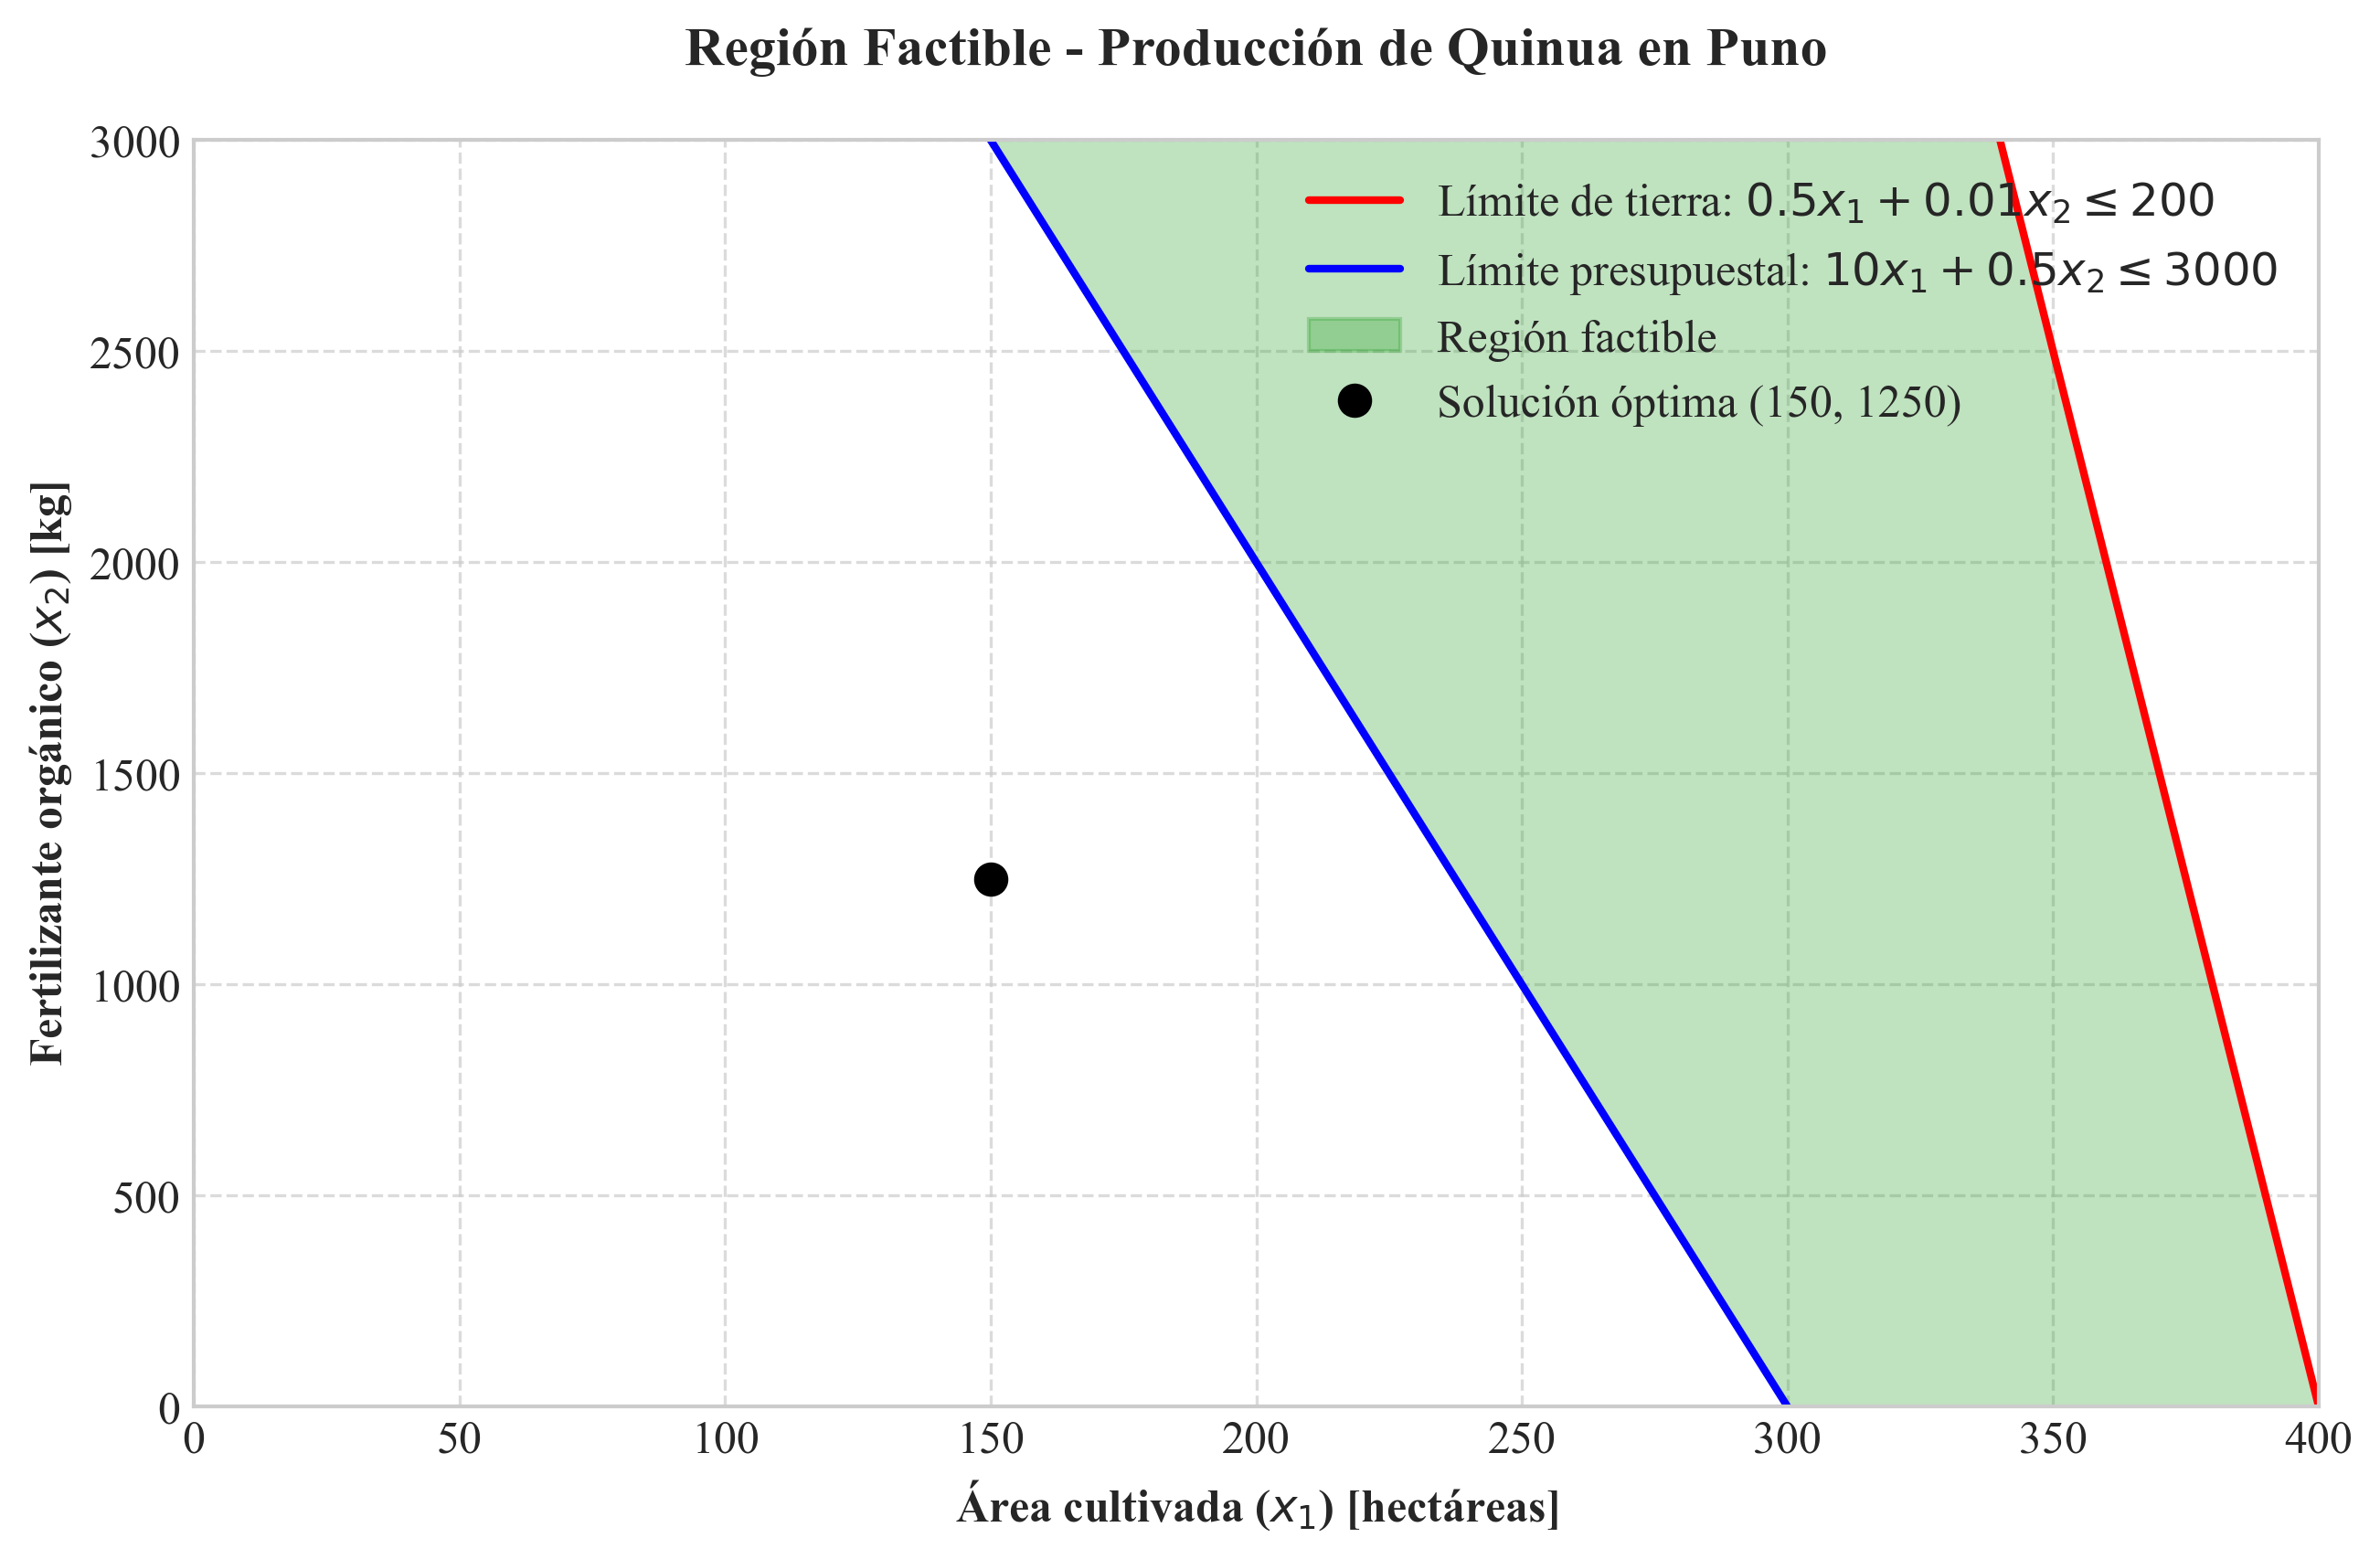
\includegraphics[width=0.8\textwidth]{region_factible_quinua.png}
\caption{Región factible del modelo (adaptado de \cite{condori2024})}
\label{fig:region}
\end{figure}

\section{Resultados}
La solución óptima reportada en \cite{condori2024} es:
\begin{align*}
x_1^* &= 150\ \text{ha} \\
x_2^* &= 1250\ \text{kg} \\
x_3^* &= 375\ \text{horas} \\
Z^* &= 215,\!625\ \text{soles}
\end{align*}

\bibliographystyle{plain}
\bibliography{referencias}

\end{document}
